% RESULTS - AUTO-UPDATED SECTION
% This section is scaffolded for the RQ-driven paper suite.
% It will be populated with findings once experiments run.

\newcommand{\pl}[1]{\textcolor{gray}{#1}}

\subsection{Overview}

We present results from the curated paper suite (baseline, calibration, ablations, sensitivity,
and RQ-specific experiments). Table~\ref{tab:summary} provides a high-level overview.

\begin{table}[htbp]
\centering
\caption{Summary of experimental results (placeholder)}
\label{tab:summary}
\begin{tabular}{lrrr}
\toprule
Experiment & Configurations & Total Runs & Key Finding \\
\midrule
\pl{Baseline} & \pl{--} & \pl{--} & \pl{TBD} \\
\pl{Calibration} & \pl{--} & \pl{--} & \pl{TBD} \\
\pl{Ablation} & \pl{--} & \pl{--} & \pl{TBD} \\
\pl{Sensitivity} & \pl{--} & \pl{--} & \pl{TBD} \\
\bottomrule
\end{tabular}
\end{table}

% ============================================================================
\subsection{RQ1: Participation Dynamics}
% ============================================================================

\subsubsection{Findings}

\begin{figure}[htbp]
    \centering
    
\includegraphics[width=0.8\textwidth]{figures/rq1_turnout}
    \caption{Turnout as a function of participation targets (placeholder).}
    \label{fig:rq1-turnout}
\end{figure}

\begin{figure}[htbp]
    \centering
    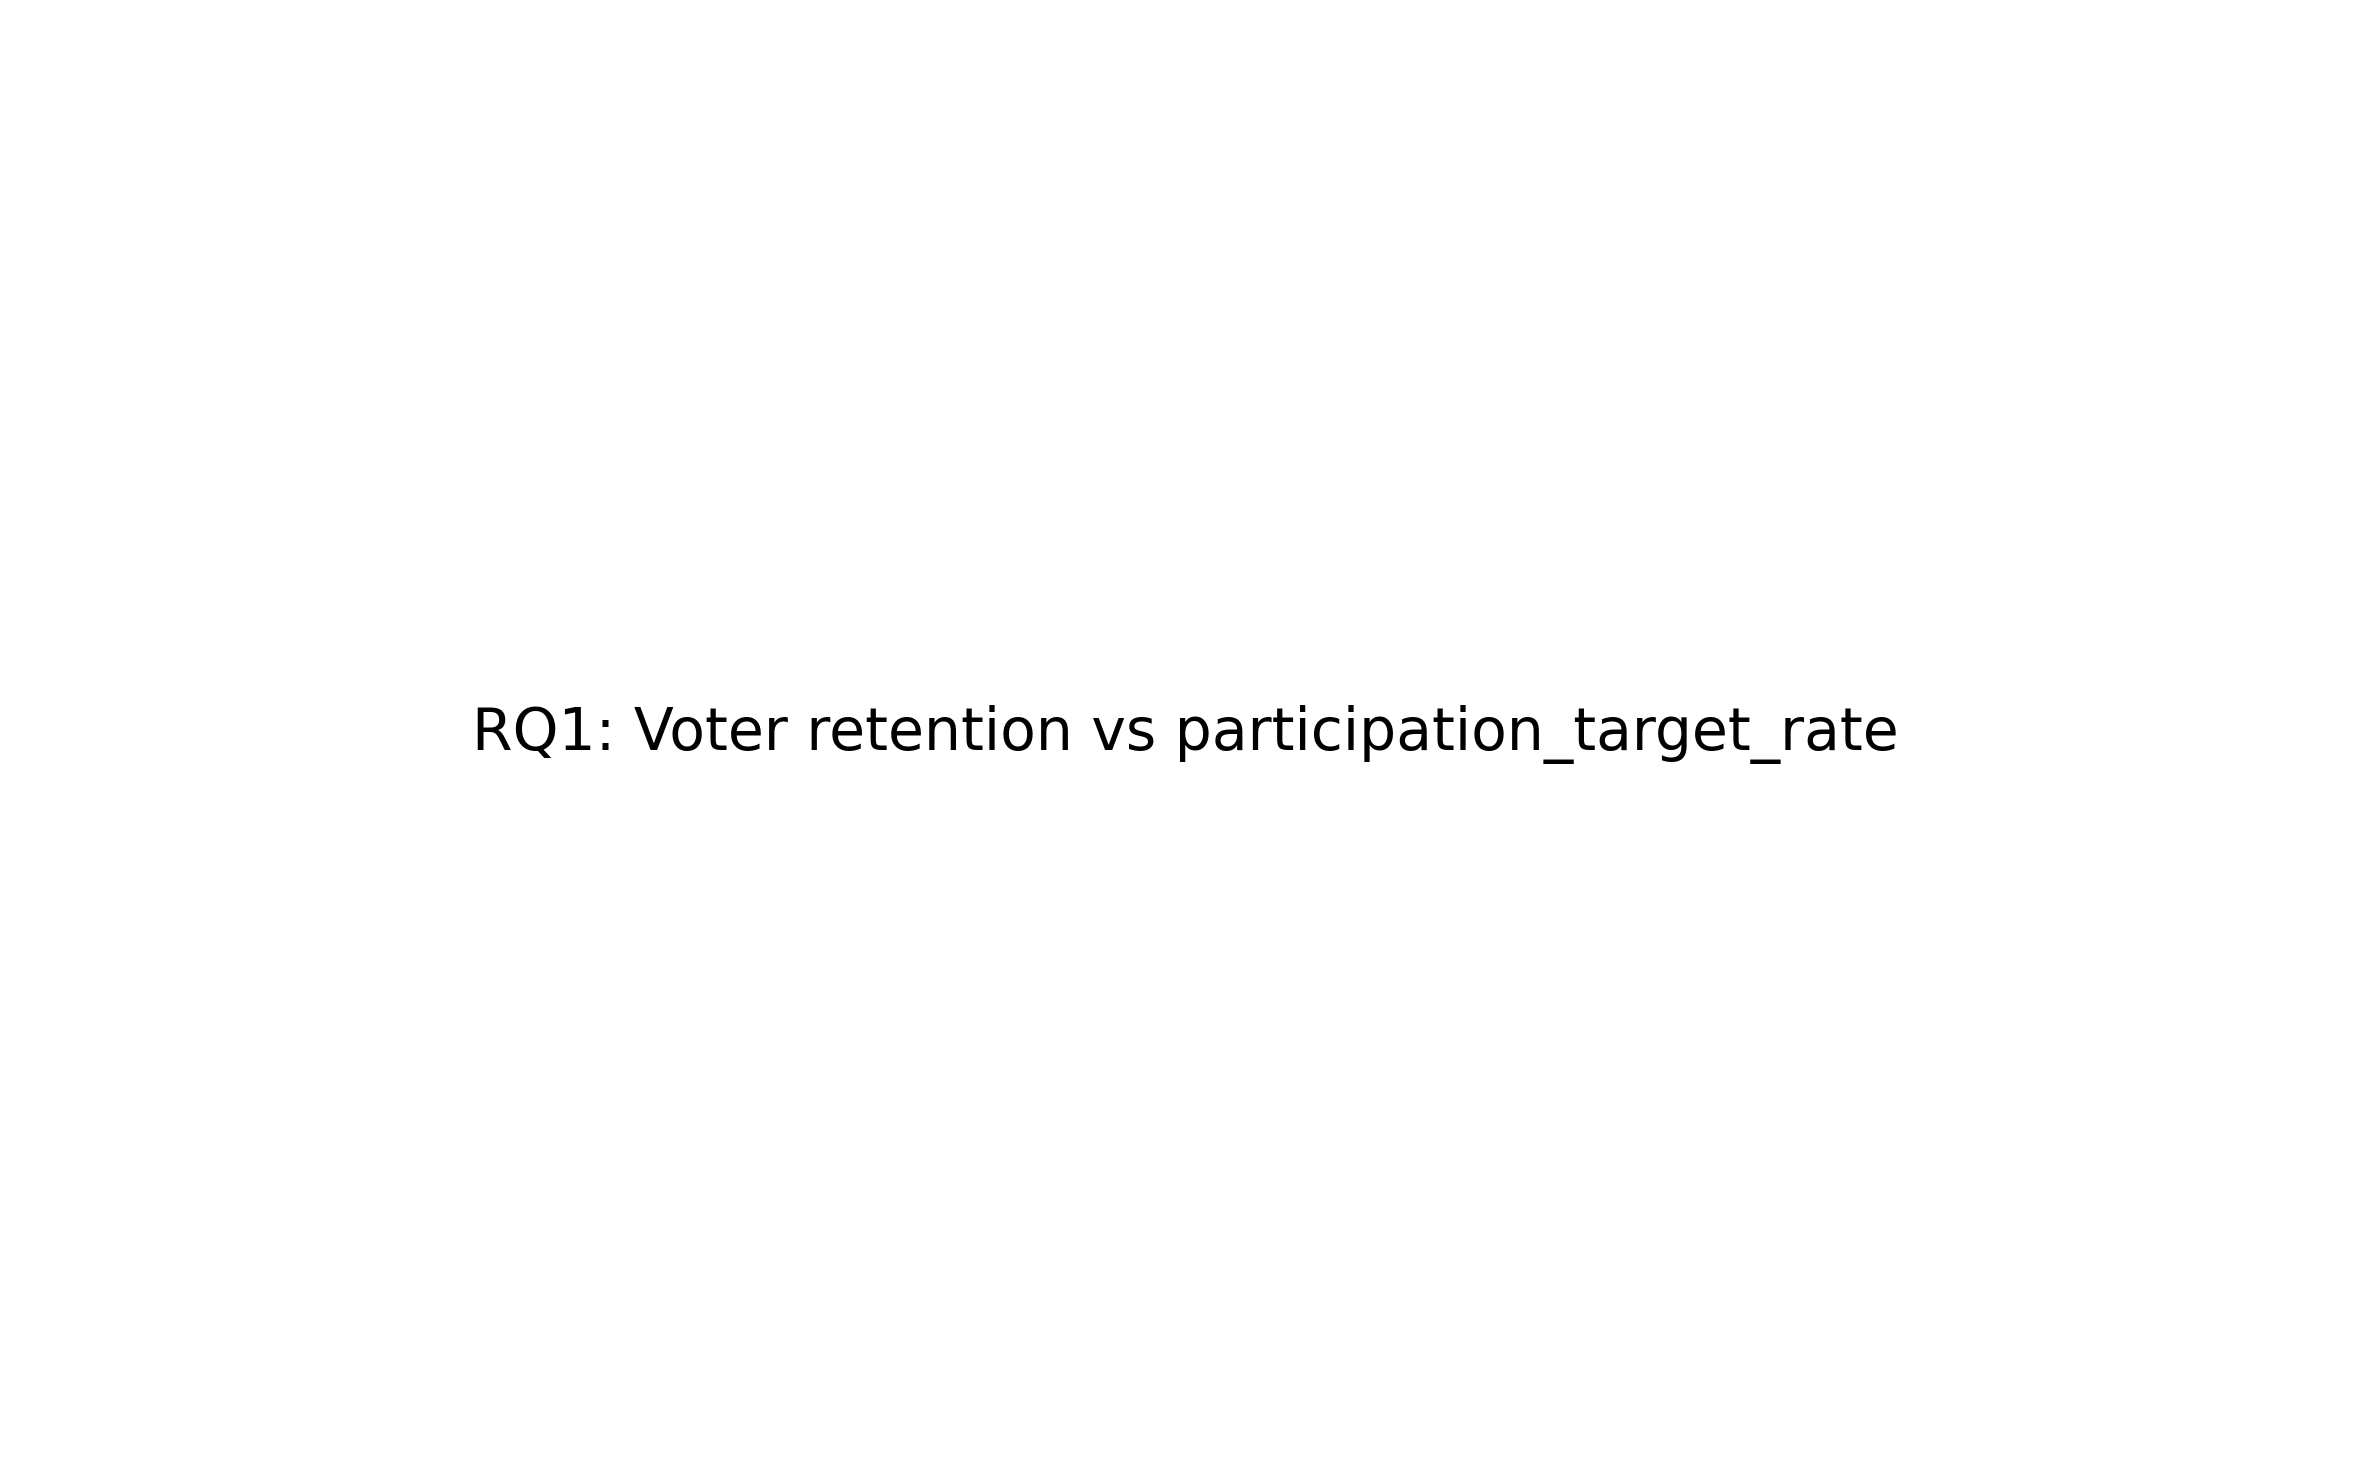
\includegraphics[width=0.8\textwidth]{figures/rq1_retention}
    \caption{Voter retention vs participation targets (placeholder).}
    \label{fig:rq1-retention}
\end{figure}

\begin{table}[htbp]
\centering
\caption{RQ1 summary stats (placeholder)}
\label{tab:rq1-summary}
\begin{tabular}{lccc}
\toprule
Metric & Mean & Std & 95\% CI \\
\midrule
\pl{Turnout} & \pl{--} & \pl{--} & \pl{--} \\
\pl{Quorum reach} & \pl{--} & \pl{--} & \pl{--} \\
\pl{Retention} & \pl{--} & \pl{--} & \pl{--} \\
\bottomrule
\end{tabular}
\end{table}

% ============================================================================
\subsection{RQ2: Governance Capture Mitigation}
% ============================================================================

\subsubsection{Findings}

\begin{figure}[htbp]
    \centering
    
\includegraphics[width=0.8\textwidth]{figures/rq2_whale_influence}
    \caption{Whale influence across mitigation settings (placeholder).}
    \label{fig:rq2-whale-influence}
\end{figure}

\begin{figure}[htbp]
    \centering
    
\includegraphics[width=0.8\textwidth]{figures/rq2_tradeoff}
    \caption{Capture risk vs throughput (placeholder).}
    \label{fig:rq2-tradeoff}
\end{figure}

\begin{table}[htbp]
\centering
\caption{Top mitigation configs (placeholder)}
\label{tab:rq2-top-configs}
\begin{tabular}{lccc}
\toprule
Config & Capture Risk & Throughput & Notes \\
\midrule
\pl{A} & \pl{--} & \pl{--} & \pl{--} \\
\pl{B} & \pl{--} & \pl{--} & \pl{--} \\
\pl{C} & \pl{--} & \pl{--} & \pl{--} \\
\bottomrule
\end{tabular}
\end{table}

% ============================================================================
\subsection{Baseline and Robustness}
% ============================================================================

\begin{table}[htbp]
\centering
\caption{Baseline headline metrics (placeholder)}
\label{tab:baseline-summary}
\begin{tabular}{lccc}
\toprule
Metric & Mean & Std & Notes \\
\midrule
\pl{Pass Rate} & \pl{--} & \pl{--} & \pl{--} \\
\pl{Turnout} & \pl{--} & \pl{--} & \pl{--} \\
\pl{Treasury Volatility} & \pl{--} & \pl{--} & \pl{--} \\
\bottomrule
\end{tabular}
\end{table}

\begin{figure}[htbp]
    \centering
    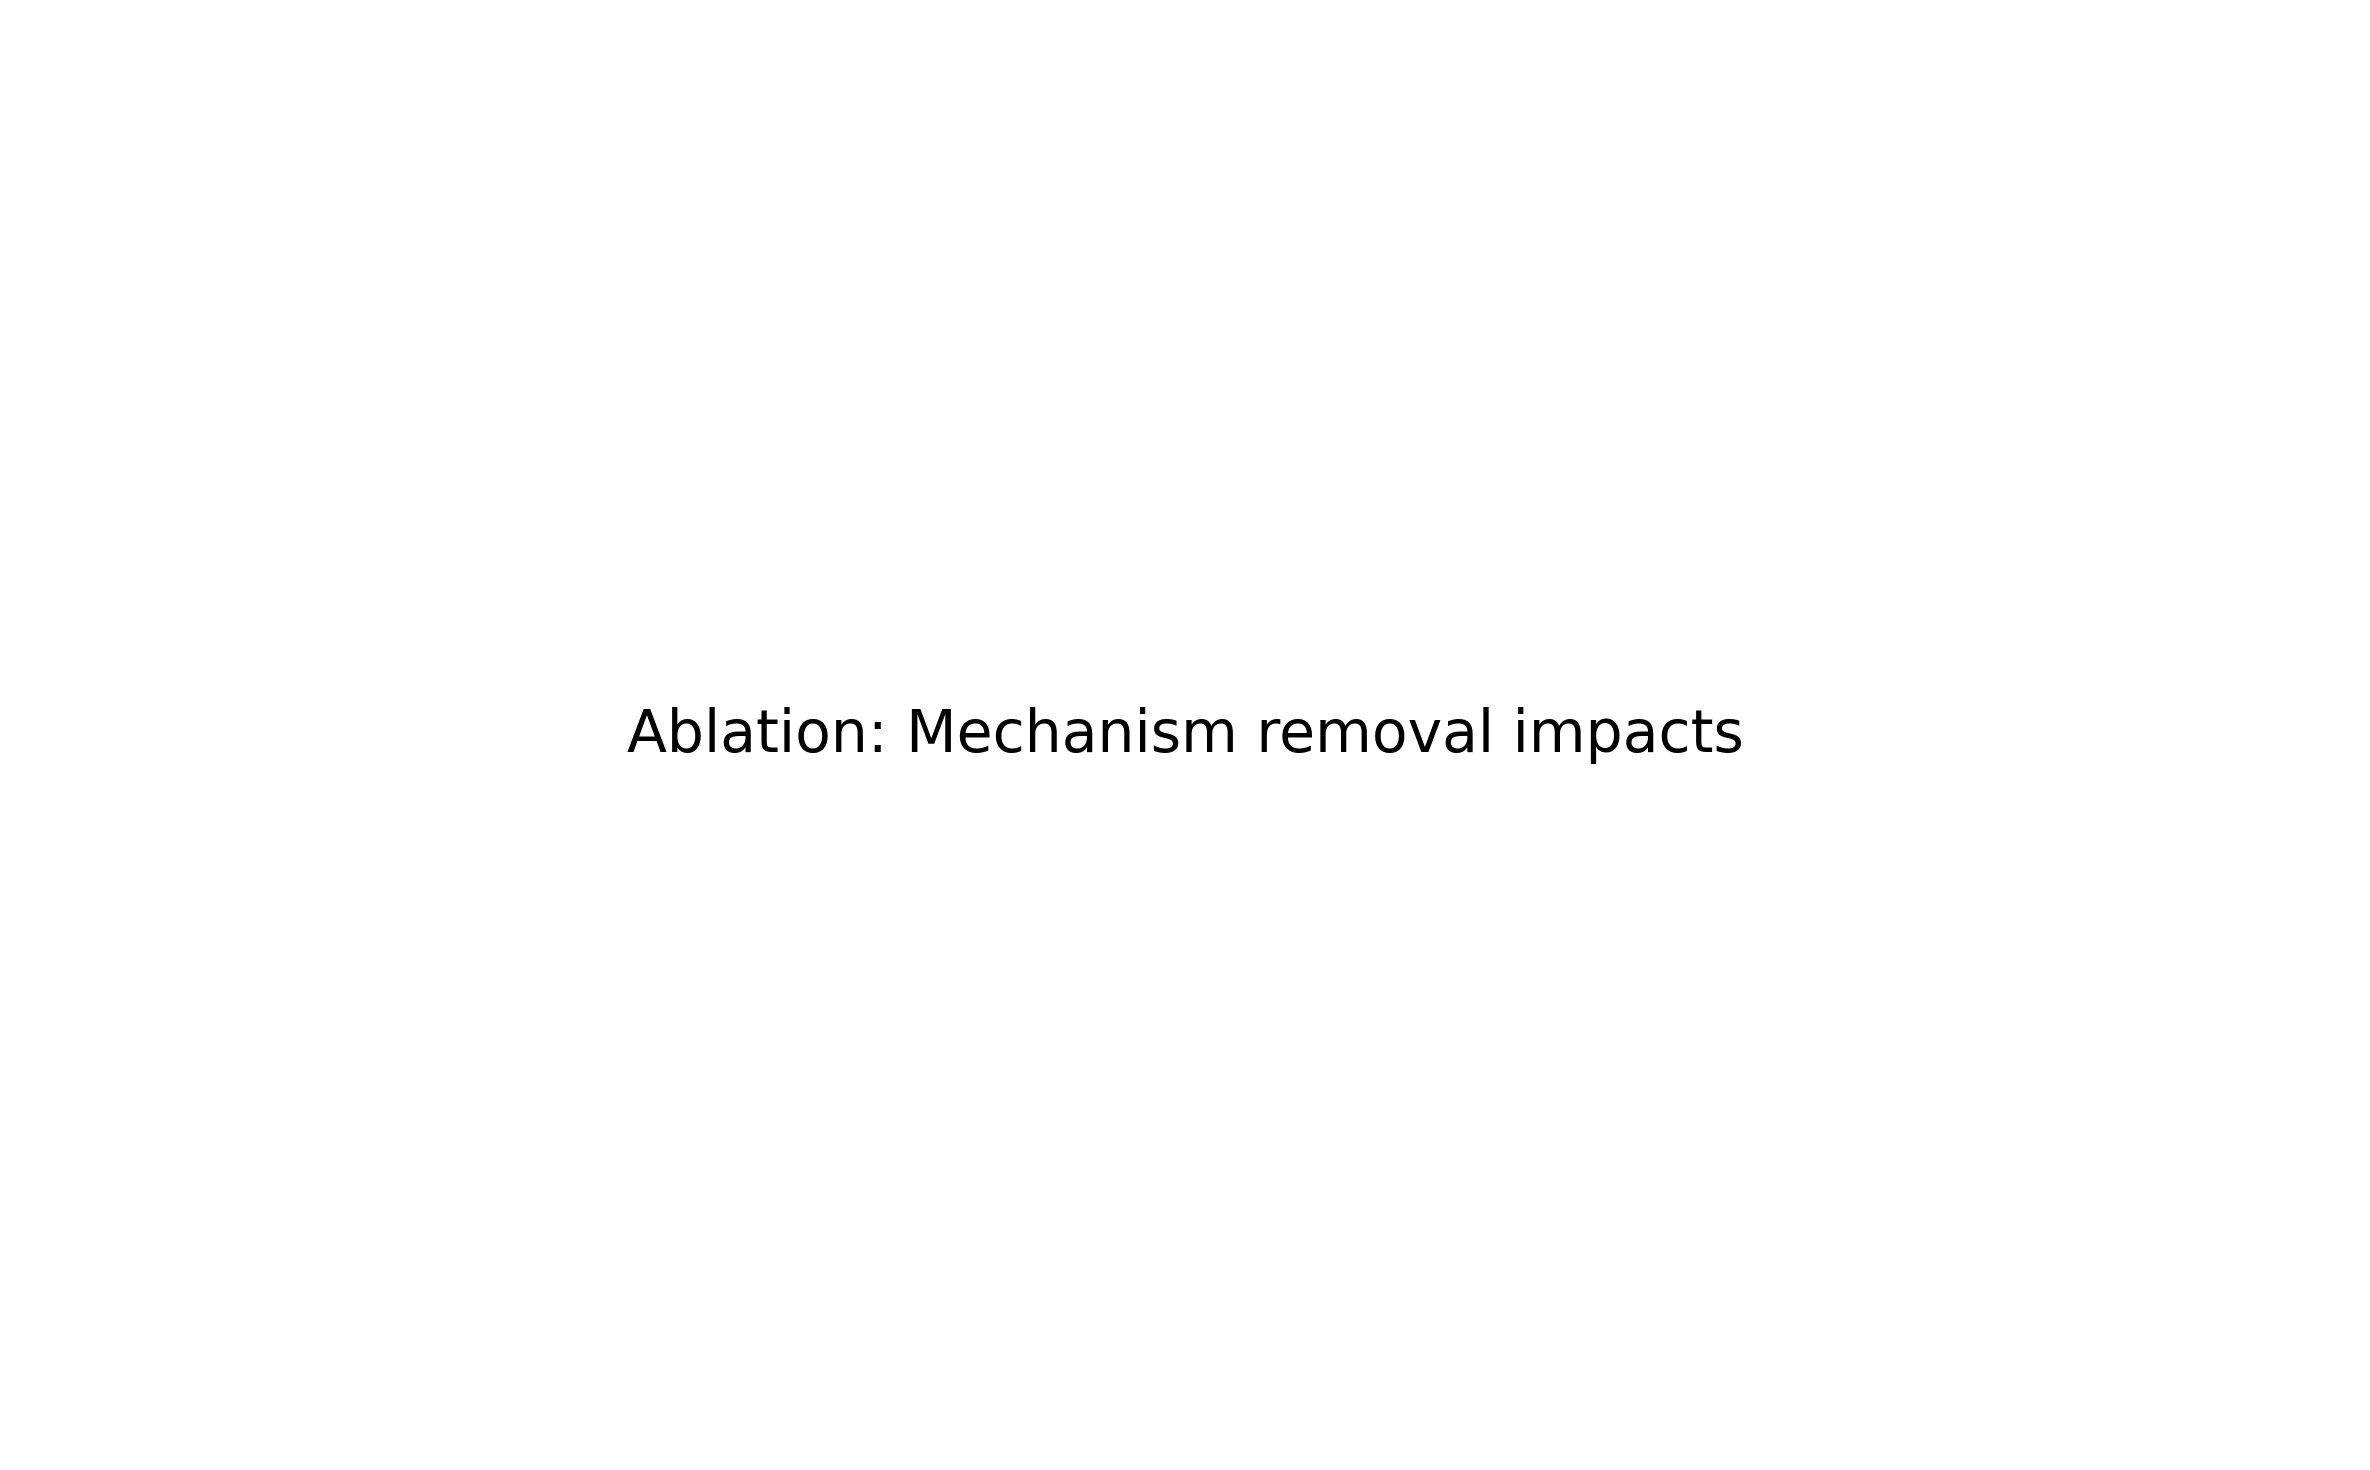
\includegraphics[width=0.8\textwidth]{figures/ablation_impact}
    \caption{Ablation impacts on governance outcomes (placeholder).}
    \label{fig:ablation-impact}
\end{figure}

\begin{figure}[htbp]
    \centering
    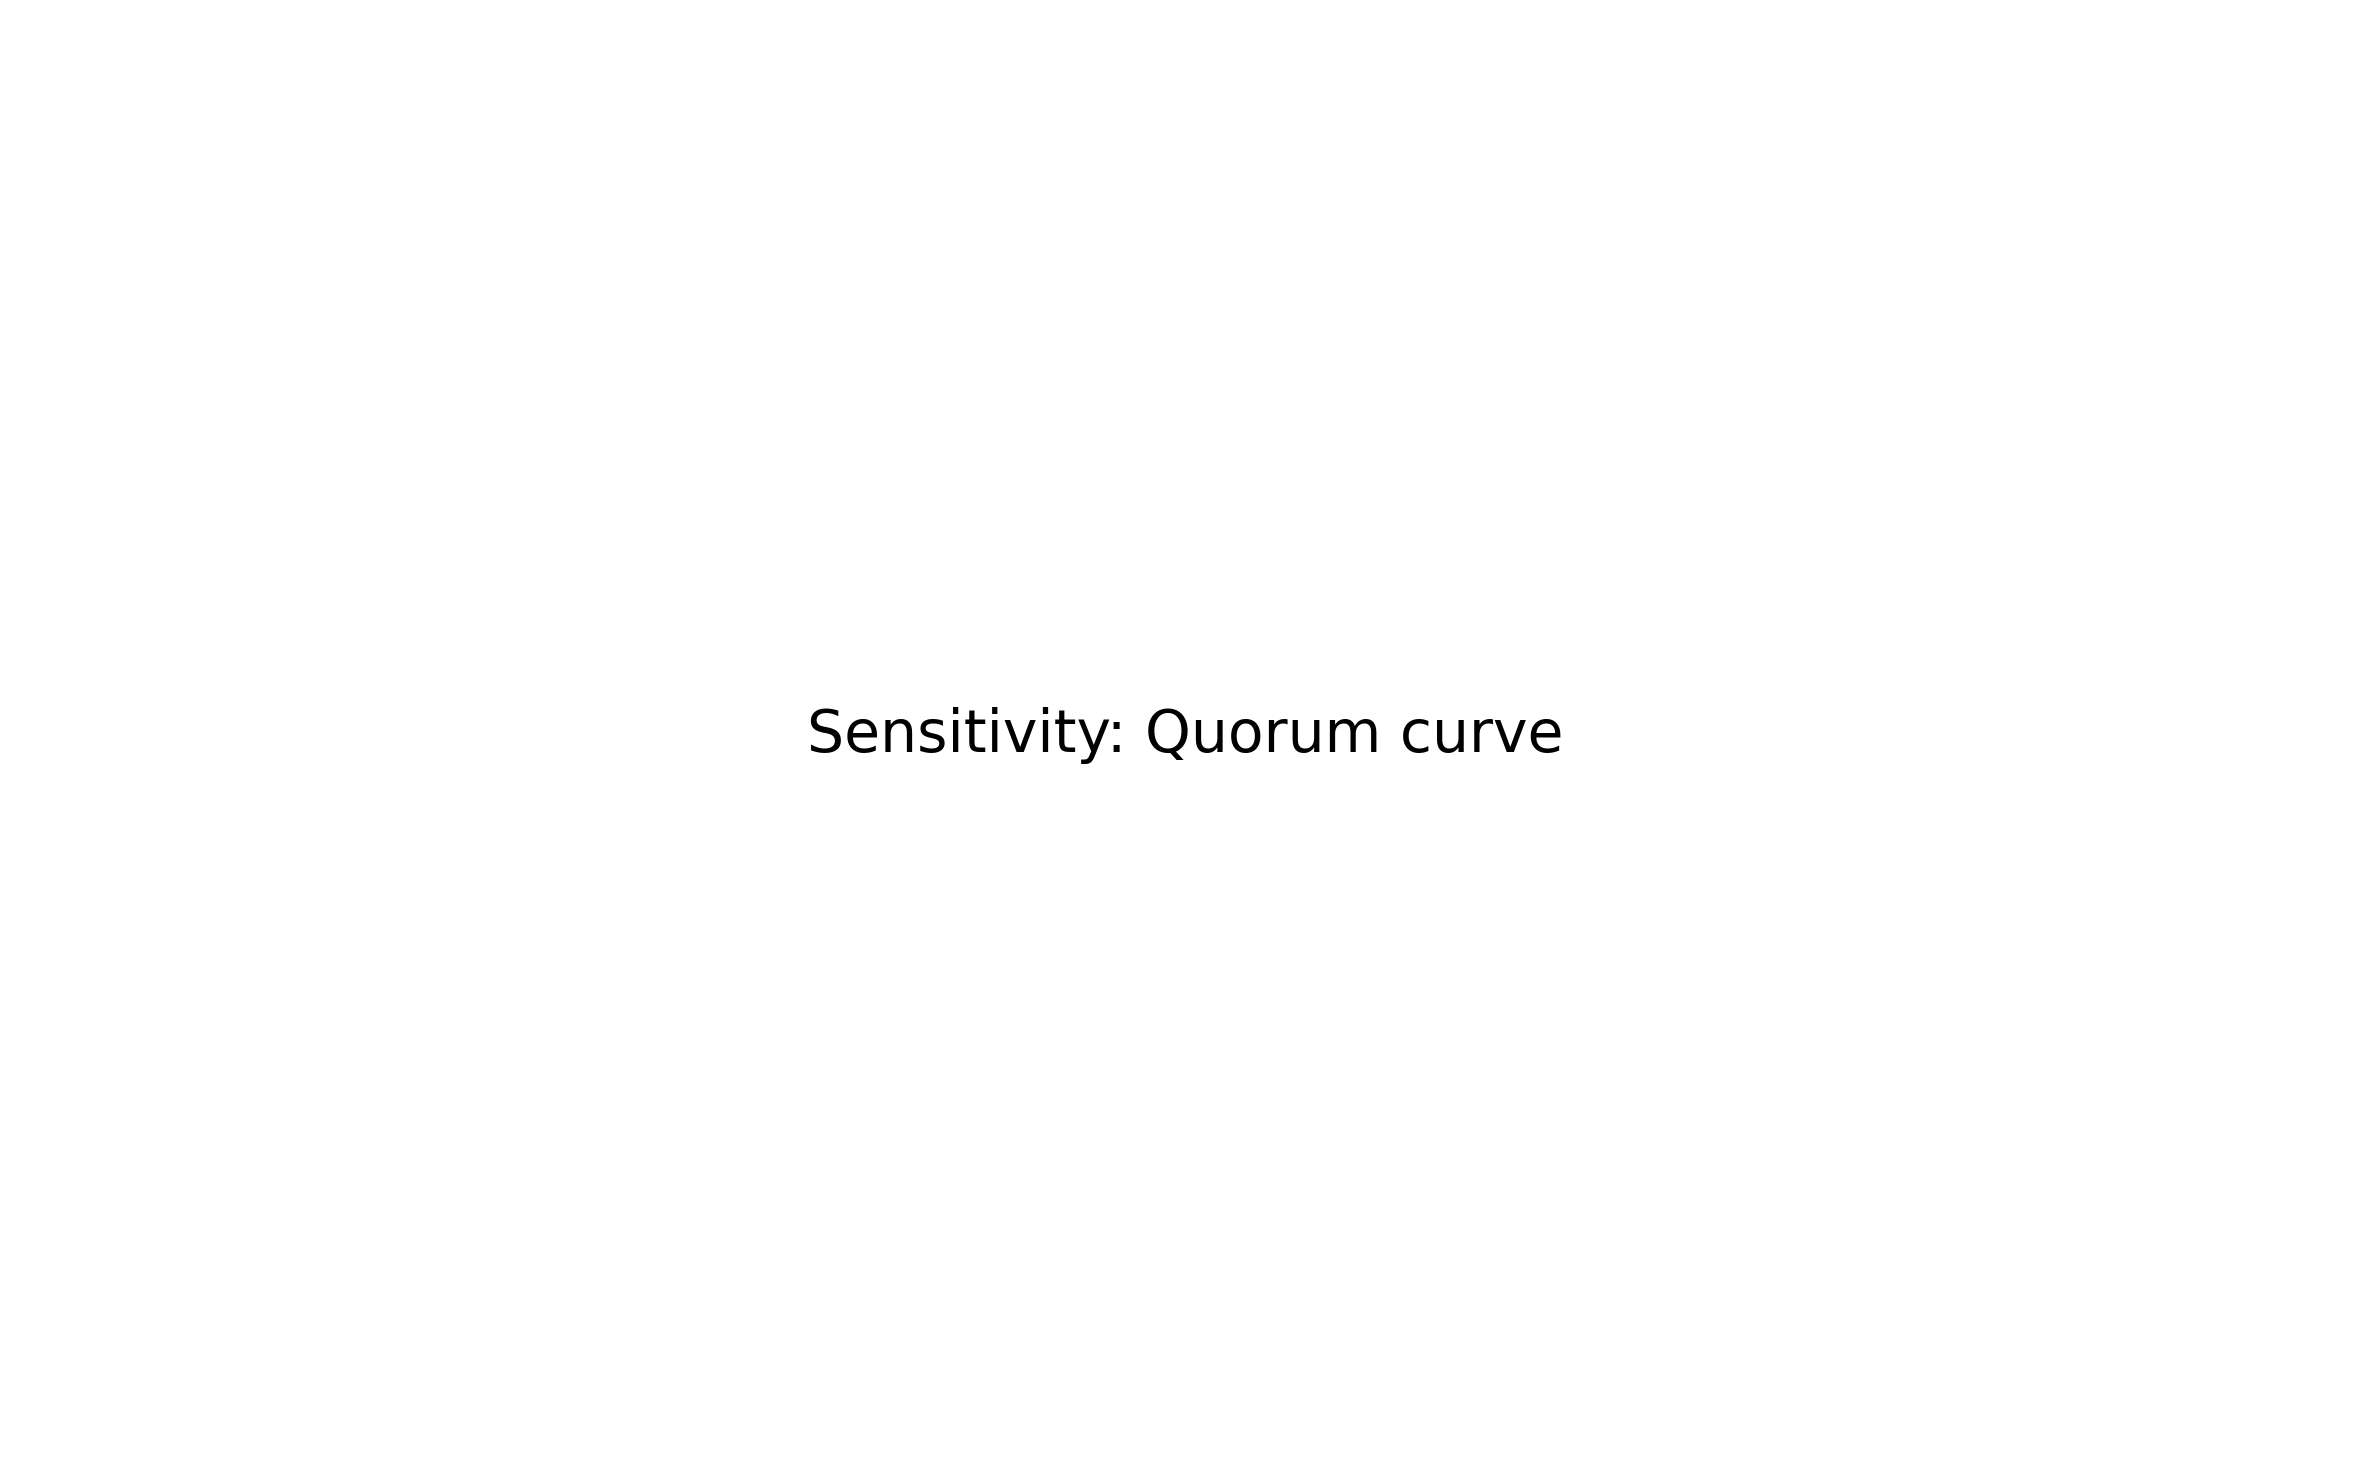
\includegraphics[width=0.8\textwidth]{figures/quorum_sensitivity}
    \caption{Quorum sensitivity curve (placeholder).}
    \label{fig:quorum-sensitivity}
\end{figure}

% === AUTO-GENERATION METADATA ===
% Regenerate this section:
%   npm run paper:update -- --section results
% Source experiments: paper suite (placeholders until runs complete)
